% THIS IS A LATEX TEMPLATE FILE FOR PAPERS INCLUDED IN THE
% *Anthology of Computers and the Humanities*.
% DO NOT change the documentclass
\documentclass[final]{anthology-ch} % for the final version

% LOAD LaTeX PACKAGES
\usepackage{booktabs}
\usepackage{graphicx}

% TITLE OF THE SUBMISSION
\title{Reconstructing Historical Events with CIDOC CRM}

% AUTHOR AND AFFILIATION INFORMATION
\author[1]{Yu Lee An}[
  orcid=0000-0001-8608-5583
]

\affiliation{1}{School of Information and Library Science, University of North Carolina at Chapel Hill}

% KEYWORDS
\keywords[eng]{temporal uncertainty, CIDOC CRM, semantic web, RDF, event modeling, historical data, British music trade, ontology}

% METADATA FOR THE PUBLICATION
% This will be filled in when the document is published; the values can
% be kept as their defaults when the file is submitted
\pubyear{2026}
\pubvolume{5}
\pagestart{38}
\pageend{47}
\paperorder{5}
\conferencename{From Manuscript to Megabyte: Building Sustainable and Open Futures in the Digital Humanities}
\conferenceeditors{James B. Harr III, Emma Stanley, Jenna Rinalducci, and Donna Kain}
\doi{10.63744/AfxZkbfK4dXG}
\customhead{}

\addbibresource{bibliography.bib}

%%%%%%%%%%%%%%%%%%%%%%%%%%%%%%%%%%%%%%%%%%%%%%%%%%%%%%%%%%%%%%%%%%%%%%%%%%%
% HERE IS THE START OF THE TEXT
\begin{document}

\maketitle

\begin{abstract}
Historical sources frequently contain uncertain, approximate, and ambiguous temporal information, posing a significant challenge for their representation in computational systems. This paper addresses this challenge by demonstrating how semantic web technologies and an event-centric ontology can systematically represent the pervasive temporal uncertainty inherent in primary sources. Using the CIDOC CRM ontology, this study outlines a structural approach to transforming linear historical narratives into explicit, machine-interpretable graphs. Drawing on the professional and commercial networks of the Georgian and Victorian British music trade as a case study, the paper identifies five distinct forms of temporal uncertainty: circa dates, bounded dates, time-spans, relative dates, and inherently fuzzy historical eras. Through the strategic interplay of CIDOC CRM's four temporal boundary properties (P82a, P81a, P81b, and P82b), the paper demonstrates how varying levels of temporal precision and modeling-imposed constraints can coexist within a single interval-based representation. Ultimately, this research argues that formalizing temporal uncertainty into explicit semantic statements does not flatten humanistic nuance. Instead, it provides a structural framework that makes complex historical data actionable for advanced workflows, such as automated reasoning and large-scale pattern analysis.
\end{abstract}

\section{Introduction} \label{sec:intro}

As computational methods become increasingly embedded in humanities research, scholars have been compelled to reconsider how historical knowledge is structured and represented. This paper contends that data modeling does more than organize historical information consistently and transparently; it actively enables new forms of research by making historical evidence amenable to computational analysis and interpretation. Such a shift challenges traditional humanistic approaches to evidence and narrative, inviting scholars to rethink the relationship between interpretation and formal representation.

This growing reliance on computational methods raises a fundamental epistemological tension between interpretive practice and computational formalization. Elena Pierazzo highlights this tension, asserting that \enquote{to compute, we need to model, and we need to do it formally, explicitly, and accurately, as sloppiness or fuzziness strongly limits the potentials of the kind of process operated by machines}~\cite[120]{pierazzo2019subjective}. From this perspective, computational processing requires historians to translate uncertainty into structured, explicit representations, approaching what Pierazzo calls a \enquote{deterministic certainty}~\cite[120]{pierazzo2019subjective}.

Johanna Drucker, on the other hand, emphasizes that humanistic data is not observer-independent, unlike data in the natural and social sciences. Nevertheless, she argues that this does not exclude such data from computation. Instead, its complexity \enquote{requires the same mathematical and computational models as other complex systems}~\cite[para.~18]{drucker2011humanities}. For Drucker, the goal is not to eliminate interpretation, but rather to encode it within a \enquote{humanistic interpretative frame that computational systems can meaningfully process}~\cite[para.~49]{drucker2011humanities}.

Both Pierazzo and Drucker, in different ways, highlight the challenges and possibilities of representing ambiguity and uncertainty in historical data computationally. A central challenge concerns temporal uncertainty, which makes computational approaches to organizing and interpreting sources particularly valuable. Given these uncertainties, subjectivities, and gaps in the historical record, historians have often privileged narrative over formal modeling, as narrative allows them to convey the layered meanings embedded in historical sources. In response, this study draws on Semantic Web technologies, which enable the explicit encoding of meaning in machine-readable form and support the integration and reuse of data across heterogeneous sources.

Using the Georgian and Victorian British music trade as a case study, this paper demonstrates how semantic modeling and computational methods can facilitate the analysis of historical events characterized by temporal uncertainty. The goal is to show how such methods transform both the representation and the interpretation of historical evidence.

\section{About the Data} \label{sec:data}

Members of the British music trade included music publishers, engravers, music sellers, musical instrument makers, and accessory makers---in short, anyone participating in the trade. The data describes connections among music traders, capturing successor--predecessor and family relationships, business associations, and the events that shaped their professional lives.

The dataset covers events tied to individuals in the trade during the Georgian and Victorian eras. Reconstruction of their activities draws on diverse primary and secondary sources, including newspaper advertisements, \textit{London Gazette} legal notices, personal correspondence, music publishers' catalogs, and Stationers' Hall registers, which recorded publications entered for copyright protection.

These events fall into four main categories. Life events include milestones such as birth, marriage, death, career changes, and relocations, providing context beyond business activities. Critical business events mark significant changes, including the formation of new partnerships, the purchase of the stock-in-trade of other music sellers, and business closures, all of which signal strategic shifts. Everyday business events encompass routine commercial and professional activities such as music printing, publishing, and engraving; musical instrument making, selling, and hiring out, placing newspaper advertisements for new publications, and maintaining circulating music libraries. Although individually minor, these activities collectively reveal long-term patterns in the music trade. Business failure events include bankruptcy, insolvency, and imprisonment for debt, financial loss and bankruptcy discharges. Together, these four categories capture the range of events that shaped music traders' lives and professional activities in Georgian and Victorian Britain.

\section{How Semantic Web Technology Can Help} \label{sec:semweb}

Semantic Web technologies can help historians by providing ways to encode data with precise contexts---embedding the meaning of every event, entity and relationship directly into the data itself. As Albers, Große, and Wagner observe, semantic modeling is the key to connecting the data content and the context~\cite[239]{albers2020semantic}. This is achieved by translating implicit, ambiguous human-language knowledge into explicit, machine-interpretable representations, shifting part of the information-processing burden from humans to machines.

Central to this approach is the Resource Description Framework (RDF), which represents information as an interrelated graph structure. As Martin, Szekely, and Allemang note, \enquote{A graph is the lowest common denominator for data representation,} and \enquote{is not limited to a particular shape}~\cite[16]{martin2021rise}. As such, it provides a universal form capable of describing a wide variety of entity types, attributes, and relationships with full fidelity. Graphs provide expressive power for modeling complex scenarios and indirect relationships that are difficult to capture with relational database models, and they scale naturally as datasets grow. Creating a complex semantic model is now feasible through both commercial and non-proprietary graph databases and graph processing software, making semantic web technologies increasingly accessible to non-technical domain experts~\cite[vii]{kejriwal2019domain}.

Open standards such as RDF Schema (RDFS), the Web Ontology Language (OWL), and the SPARQL Protocol and RDF Query Language (SPARQL) further enable interoperability among datasets and support the linking of related information across heterogeneous sources. Additionally, RDF reification allows scholars to represent multiple interpretations and record the provenance of historical information through formal vocabularies and ontologies~\cite[54, 57]{allemang2020semantic}\cite[81-82]{hogan2020web}, thereby supporting the integration of data-driven approaches with traditional narrative history.

\section{Modeling} \label{sec:modeling}

Events in the British music trade can be modeled as RDF triples, forming a graph using the event-oriented CIDOC CRM ontology developed by the International Council of Museums (CIDOC). CIDOC CRM is widely used in the cultural heritage sector and is particularly well-suited for modeling historical data. This research employs the Erlangen CIDOC CRM, an RDF Schema expression of the CRM~\cite{doerr2020implementing}. CIDOC CRM treats events as primary entities.

Modeling historical events involves defining and relating entities through their temporal relationships---a process complicated by pervasive uncertainty. The National History Standards state, \enquote{Chronology provides the mental scaffolding for organizing historical thought}~\cite[7]{nationalhistory1995standards}. But historians' scaffolding is often unstable. Historian David Fischer warns against the \enquote{fallacy of misplaced precision}~\cite[61]{fischer1970historians}, emphasizing that overstating empirical certainty is problematic. Effective modeling, therefore, formalizes uncertainty rather than eliminating it, enabling machines to process uncertainty through logic-based languages. By encoding these uncertainties, historians can better manage inherent ambiguities.

Within the CIDOC CRM framework, the \texttt{E5\_Event} class serves as the structural nexus connecting diverse historical entities. To illustrate: the 1781 keyboard duel between Mozart and Clementi---arranged by Emperor Joseph II of Austria at the Viennese court~\cite[357]{desaintfoix1923muzio}---is modeled as an \texttt{E5\_Event} (see Figure~\ref{fig:duel-graph}). Often referred to as the \enquote{Clementi--Mozart duel,} the event was a keyboard competition in the presence of Emperor Joseph II, the Grand Duke Paul of Prussia, Grand Duchess Maria Fyodorovna of Prussia, and members of the imperial court. During the evening, the two musicians performed solo works, improvised at the keyboard, and participated in a two-piano performance. Although the contest was officially declared a draw, it became one of the celebrated musical events of the late eighteenth century.

The relevant actors---Mozart, Clementi, the Emperor, and the Duke and Duchess of Prussia---are represented as instances of \texttt{E39\_Actor}; the event's date, December 24, 1781, as an \texttt{E52\_Time-Span}; and the Imperial Court in Vienna as an \texttt{E53\_Place}. The \texttt{E5\_Event} acts as the central hub, using semantic properties such as \texttt{P12\_occurred\_in\_the\_presence\_of}, \texttt{P7\_took\_place\_at}, and \texttt{P4\_has\_time-span} to integrate distinct entities into a structured, machine-interpretable graph.

While humans may effortlessly synthesize the Mozart and Clementi piano duel into a single mental image, computational systems require this event to be decomposed into explicit data connections. Computational systems cannot reliably infer implicit relationships unless these are encoded as structured data elements. By representing events as distinct entity nodes and applying properties such as \texttt{P12\_occurred\_in\_the\_presence\_of} (linking \texttt{E39\_Actor}) and \texttt{P7\_took\_place\_at} (linking \texttt{E53\_Place}), a linear historical narrative is transformed into a highly contextualized graph. This approach yields a model representing entities, events, and a network of relationships---including those involving music publishers, printers, instrument makers, and other participants.

\begin{figure}[t!]
  \centering
  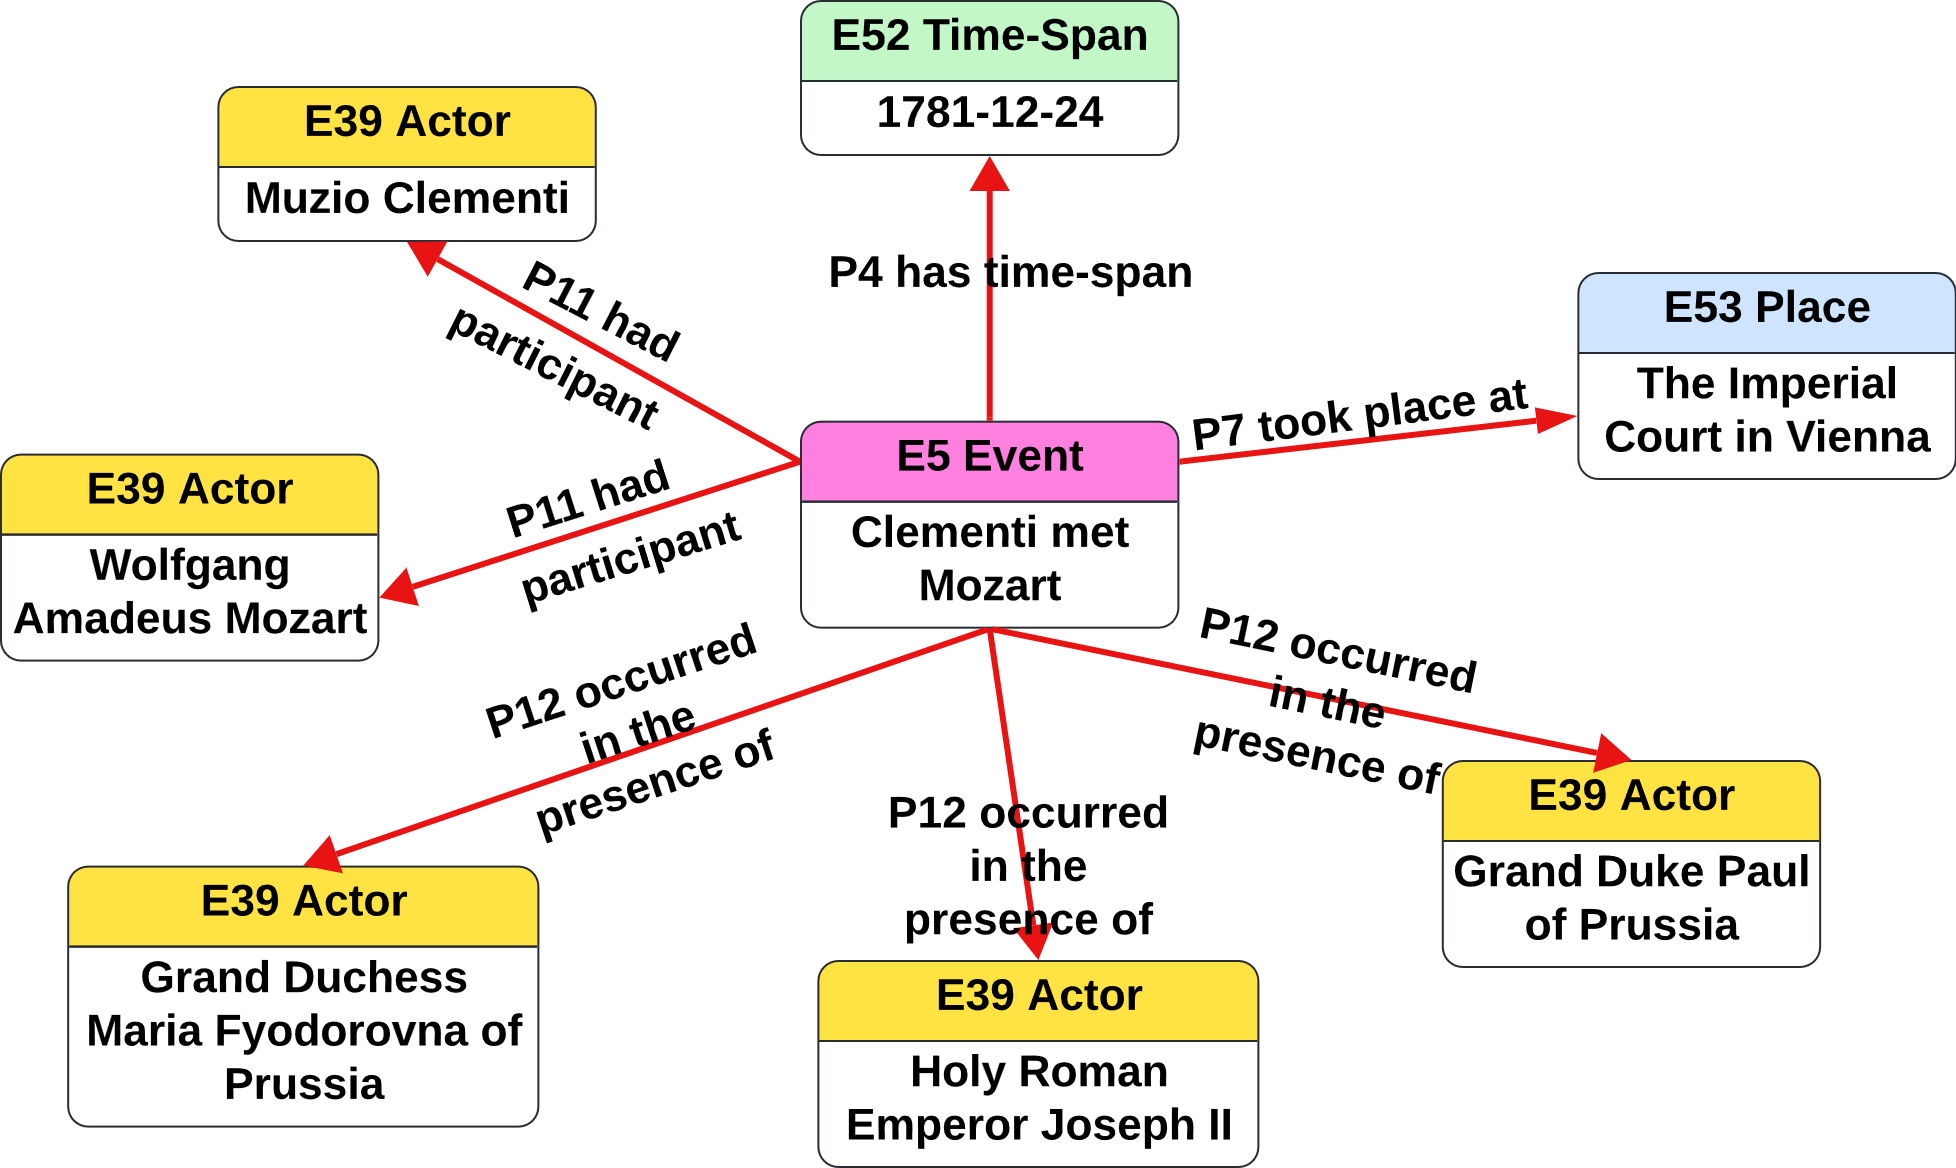
\includegraphics[width=0.9\linewidth]{images/figure1_duel_graph.png}
  \caption{The 1781 musical encounter between Muzio Clementi and Wolfgang Amadeus Mozart, expressed in CIDOC CRM.}
  \label{fig:duel-graph}
\end{figure}

The diagram in Figure~\ref{fig:duel-graph} represents the following elements:
\begin{itemize}
  \item \texttt{E5\_Event}: the overarching event itself---the duel/meeting.
  \item \texttt{E39\_Actor}: the people involved---Mozart, Clementi, the Emperor, and the Duke and Duchess of Prussia.
  \item \texttt{E53\_Place}: where it happened (the Austrian Court/Palace).
  \item \texttt{E52\_Time-Span}: when it happened (December 24, 1781).
  \item \texttt{P12\_occurred\_in\_the\_presence\_of}: the semantic property linking the event to the actors who were there.
  \item \texttt{P7\_took\_place\_at}: the semantic property linking the event to its physical location.
\end{itemize}

Each triple connects actors (people or organizations), events, and places, and represents their relationships. Actor data identifies individuals or organizations and records the various roles they played, such as music publisher, engraver, seller, or musical instrument maker. Event data describes what happened and when, including time-spans. Relationship properties capture partnerships, family ties, successor-predecessor links, and broader business associations. Spatial data records business locations and changes over time. Temporal uncertainties are captured by CIDOC CRM properties.

Time itself requires careful consideration; it can be represented as either a quantitative or qualitative entity~\cite[3]{batsakis2009temporal}. When considering time quantitatively, we usually refer to either a point in time or an interval. In this study, all events are modeled as having beginnings and endings and cannot possess zero duration. This research aligns with the point of view expressed by Freksa~\cite{freksa1992temporal}, Allen~\cite{allen1983maintaining}, and Hamblin~\cite{hamblin1972instants}, asserting that representing time as truly instantaneous points with zero duration is illogical. Papadakis, Doerr and Plexousakis, too, argue that \enquote{there are no instantaneous observable phenomena}~\cite[4]{papadakis2014fuzzy}, meaning all events must have a spatio-temporal extent. This position forms the foundation for modeling time in this study.

\section{The Challenge of Representing Time in Historical Data} \label{sec:challenge}

The British music trade dataset contains numerous temporal references and modeling them presents a significant challenge because historical dates are often imprecise, incomplete, and uncertain. Although chronology is fundamental to understanding historical processes, exact dates and precise temporal boundaries are often unavailable in historical sources. Temporal information is commonly expressed through qualitative, natural-language phrases, such as \enquote{in the early days of,} \enquote{up to about,} and \enquote{was for a time.} Historians routinely interpret such expressions by drawing on contextual knowledge and linguistic cues. Computers, however, cannot reliably interpret these meanings without formal representations.

This research identifies five principal forms of temporal uncertainty.

\subsection{Circa Dates}

The first category consists of circa dates, which may be expressed numerically or in natural language. In these cases, a date is provided in the source, but some degree of uncertainty surrounds its accuracy. Examples include \enquote{about 1778,} \enquote{circa 1800,} or \enquote{near the year 1800.} Such dates establish a likely temporal reference point while acknowledging potential deviation from the stated date. When derived from reliable sources, these dates are often considered highly probable, although some uncertainty remains.

\subsection{Dates Expressed through Temporal Boundaries}

The second category includes dates qualified by expressions such as \enquote{from,} \enquote{before,} or \enquote{after} a specific date. Here, a temporal boundary is known, but the duration or extent beyond that boundary remains uncertain. For example, the phrase \enquote{from 1650 onward} establishes a lower temporal bound but does not indicate how long the associated event continued. Similar examples include \enquote{before the year xxxx,} \enquote{after xxxx,} \enquote{shortly after this date,} \enquote{prior to this time,} \enquote{sometime about or prior to the year xxxx,} and \enquote{up to about xxxx.}

\subsection{Time-Spans}

A third form of uncertainty involves time-spans, of which two distinct cases can be identified. The first concerns events known to have occurred at a particular point in time, although the exact date remains unknown: historians may know the earliest possible date (\textit{terminus post quem}) and the latest possible date (\textit{terminus ante quem}). The second case concerns events that span a period---such as wars, monarchical reigns, and large-scale social, economic, technological, and cultural transformations---in which uncertainty may exist regarding their beginning, their end, or both. One of the temporal boundaries may therefore be represented by approximate or fuzzy dates.

\subsection{Relative Dates}

A fourth category consists of relative dates, in which temporal information is defined through relationships to other events rather than through explicit calendar dates. Although the exact timing may be unknown, historians may know that event A bears temporal relation to event B, such as occurring before, after, during, overlapping with, starting, or finishing it. Such relationships are commonly analyzed using Allen's Interval Algebra~\cite{allen1983maintaining} and provide valuable temporal information even when absolute dates are unavailable.

\subsection{Inherently Fuzzy Dates}

The final category encompasses inherently fuzzy dates. Some temporal expressions, such as \enquote{at a later date} and \enquote{many years before,} lack sufficient specificity to support precise dating. More importantly, certain historical phenomena are inherently uncertain, and historians generally do not attempt to assign precise start and end dates. The Industrial Revolution provides a notable example. Historians no longer accept the view that it began suddenly in the 1750s and concluded in the 1830s; rather, they regard it as a long-term process that began earlier and extended into the early twentieth century~\cite[24-25]{berg1992rehabilitating}\cite[26]{stobart1996eighteenth}\cite[196]{withers1985mapping}. In such cases, assigning precise start and end dates is neither realistic nor historically meaningful.

Throughout the modeling process, a balance is maintained between two approaches: a conservative approach that encodes only information explicitly stated in the sources, and an interpretive approach that fills gaps using informed domain knowledge, provided such inference is supported by evidence.

\section{Modeling Temporal Uncertainty} \label{sec:modeling-uncertainty}

The preceding discussion demonstrates that historical dates are rarely precise and often appear as bounded, relative, or inherently fuzzy temporal expressions. A semantic model must therefore accommodate varying degrees of certainty rather than assume exact dates and times. CIDOC CRM is particularly well-suited to this task because it allows events and their temporal extents to be described explicitly while preserving inherent uncertainty. As an event-centric ontology, it enables the documentation not only of what occurred, but also of participants, locations, and broader interrelationships associated with an event.

\begin{sloppypar}
CIDOC CRM represents varying degrees of temporal uncertainty through the combined application of four temporal boundary properties: \texttt{P82a\_begin\_of\_the\_begin}, \texttt{P81a\_end\_of\_the\_begin}, \texttt{P81b\_begin\_of\_the\_end}, and \texttt{P82b\_end\_of\_the\_end}. The P82 pair establishes the outer limits within which an event may have occurred, while the P81 pair defines the interval during which the event is known to have been ongoing based on available evidence (see Figure~\ref{fig:timespan}). Taken together, these properties distinguish what is possible from what is certain, providing a formal mechanism for representing temporal boundaries with differing levels of precision.
\end{sloppypar}

To illustrate how CIDOC CRM represents uncertain time-spans, consider the aforementioned encounter between Wolfgang Amadeus Mozart and Muzio Clementi on Christmas Eve 1781. Although this event occurred in Vienna and predates Clementi's publishing career, it is included in the dataset because of his later prominence within the British music trade. Following his move to London, Clementi became one of the most influential music publishers, piano manufacturers, and musical entrepreneurs in Georgian London. The example illustrates how an event-centric model can capture historically significant events associated with important actors, even when those events occur outside the dataset's immediate geographical or chronological focus.

The duel also exemplifies a common type of temporal uncertainty found in historical datasets. Contemporary sources---specifically Mozart's correspondence with his father---confirm that the event took place on the evening of 24 December 1781~\cite[357]{desaintfoix1923muzio}, yet they omit the precise start and end times. The date of the event, therefore, can be established with considerable confidence (the outer boundary), while its internal temporal extent remains uncertain. Because the encounter is known to have occurred in the evening, it is reasonable to assume that the duel was ongoing between 6:00 PM (18:00:00) and 8:00 PM (20:00:00). The four temporal boundary properties mentioned above can formalize this hypothesis.

Together, these four properties define a temporal window within which the event may have occurred. They indicate that the duel was plausibly in progress between 18:00:00 and 20:00:00 while acknowledging that the exact duration cannot be determined from the available evidence. Importantly, the same four properties apply regardless of whether the temporal boundaries are uncertain or known with precision. If the event were documented to have started precisely at 18:00:00 and concluded at 20:00:00, the same four properties would be deployed. In that scenario, the values of P82a and P81a would coincide, as would the values of P81b and P82b, thereby expressing temporal certainty rather than uncertainty.

\begin{itemize}
  \item \texttt{P82a\_begin\_of\_the\_begin} = the earliest possible time (\textit{terminus post quem}).
  \item \texttt{P81a\_end\_of\_the\_begin} = the earliest confirmed time.
  \item \texttt{P81b\_begin\_of\_the\_end} = the latest confirmed time.
  \item \texttt{P82b\_end\_of\_the\_end} = the latest possible time (\textit{terminus ante quem}).
\end{itemize}

\begin{figure}[t!]
  \centering
  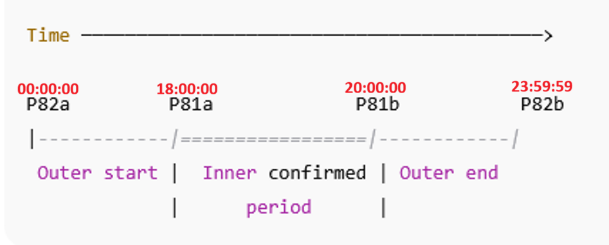
\includegraphics[width=0.85\linewidth]{images/figure2_timespan.png}
  \caption{Expressing time-span (Clementi--Mozart duel).}
  \label{fig:timespan}
\end{figure}

A different temporal structure is exhibited by the bankruptcy notice of Andrew Loder---a music seller, dealer, and chapman of Bath---published in the \textit{London Gazette}. The notice required Loder to surrender himself to the Court of Commissioners of Bankrupt at three scheduled sittings, each starting at 11:00:00 AM at the White Lion Inn in Bath (Figure~\ref{fig:loder-notice}).

In CIDOC CRM terms, each sitting is represented as an interval whose beginning is precisely specified in the source. This is encoded as a fully constrained lower boundary, where \texttt{P82a\_begin\_of\_the\_begin} and \texttt{P81a\_end\_of\_the\_begin} converge due to complete certainty about the interval's onset. However, the notice does not specify the end time of these sittings. To maintain a consistent interval structure under partial specification, this study introduces a modeling convention of a minimum duration of an hour. This is a formal constraint on the representation of temporal extents, partially derived from historical evidence of bankruptcy proceedings. Under this convention, each interval is extended by a minimum modeled duration of one hour, so \texttt{P81b\_begin\_of\_the\_end} is set to 12:00 PM for an 11:00 AM start.

Because the outer boundary is bounded at the day level, \texttt{P82b\_end\_of\_the\_end} is mapped to the final moment of the attested calendar day (i.e., 1827-03-19T23:59:59 for the first sitting). The result is an asymmetrical temporal structure in which the beginning of the event interval is precisely pinpointed to the hour, while the end remains bounded at the broader granularity of the calendar day. This configuration explicitly separates source-attested temporal information from modeling-imposed constraints. It demonstrates how CIDOC CRM accommodates hybrid temporal configurations in which varying levels of precision coexist within a single interval-based representation and are systematically expressed through the relationships between the P81 and P82 property pairs.

\begin{figure}[t!]
  \centering
  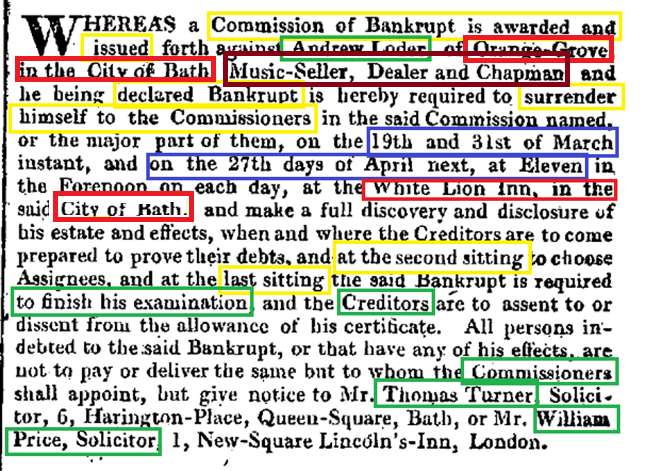
\includegraphics[width=0.75\linewidth]{images/figure3_loder_notice.png}
  \caption{Andrew Loder bankruptcy notice. \textit{London Gazette}, March 27, 1827, \url{https://www.thegazette.co.uk/London/issue/18344/page/646}. Different data elements have been color-coded: events in yellow, dates and times in blue, places in red, and actors in green.}
  \label{fig:loder-notice}
\end{figure}

\section{Conclusion} \label{sec:conclusion}

Historians encounter unique challenges as information modelers, given that documentary evidence is often scarce, fragmented, or inconclusive. Temporal uncertainty is not merely a hurdle to overcome, but an enduring aspect of reconstructing the past. This study has shown how diverse forms of temporal uncertainty---such as circa dates, dates expressed through temporal boundaries, time-spans, relative dates, and inherently vague historical periods---can be systematically formalized for computational purposes.

By utilizing the event-centric framework of CIDOC CRM---specifically, the interplay between the \texttt{P81\_ongoing\_throughout} and \texttt{P82\_at\_sometime\_within} temporal properties and their associated boundary subproperties (P81a, P81b, P82a, and P82b)---ambiguous natural language and incomplete chronological markers can be transformed into rigorous, machine-interpretable data structures without imposing unwarranted precision. The two case studies presented here, the Clementi--Mozart keyboard duel and the Andrew Loder bankruptcy notice, illustrate how this framework handles both partial and asymmetrical temporal knowledge within a consistent formal structure.

Ultimately, this modeling process is a crucial first step in making complex historical texts actionable for machine intelligence. By formalizing temporal ambiguity within a standardized ontology, historians enable advanced computational workflows---such as executing sophisticated SPARQL queries across diverse datasets, using automated reasoners to infer missing chronological connections, and analyzing long-term patterns within the music trade. Transforming temporal uncertainties in historical sources into explicit semantic RDF triples does not diminish historical nuance; rather, it supplies the computational scaffolding needed to extend humanistic interpretation into the digital era.

\begin{figure}[t!]
  \centering
  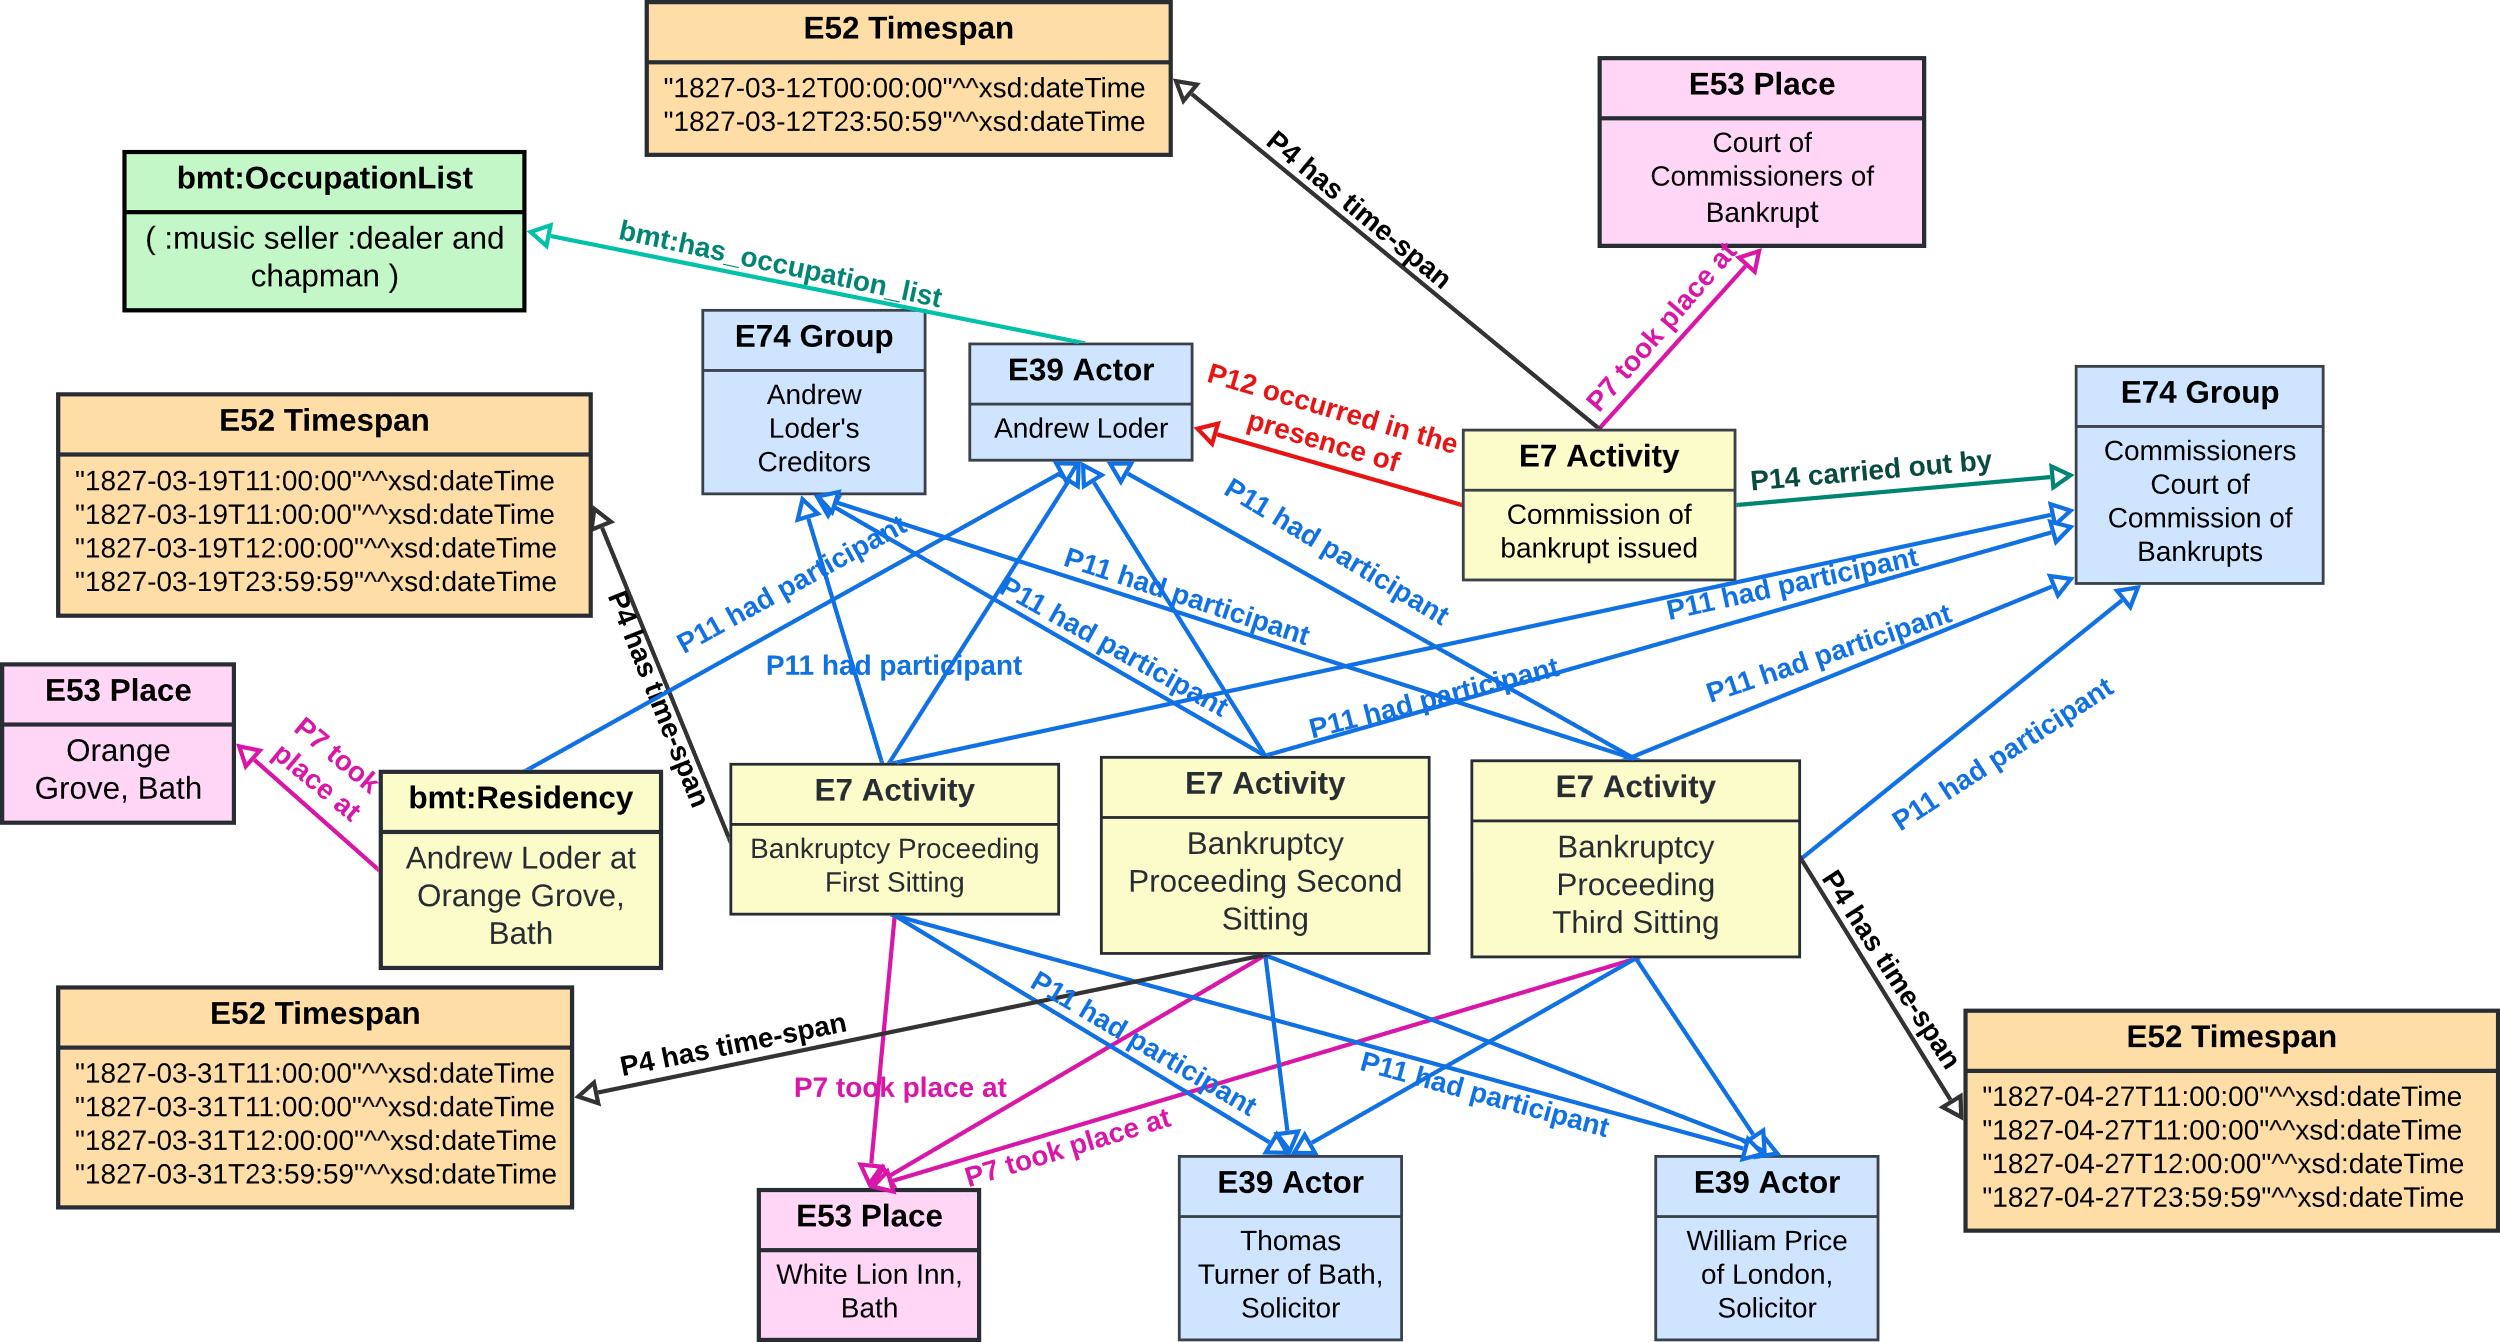
\includegraphics[width=\linewidth]{images/figure4_loder_graph.png}
  \caption{Graph representation of the Andrew Loder bankruptcy notice.}
  \label{fig:loder-graph}
\end{figure}

% Print the biblography at the end.
\printbibliography

\end{document}
